%! Author = joaos
%! Date = 15/11/2024
\pagestyle{fancy}

\newday{15 Novembro 2024}

Hoje realizou-se a lixiviação com Tiossulfato do restante material da amostra \texttt{A08.3}, a mesma utilizada na digestão ácida -~\nameref{day:8-novembro-2024}.

A lixiviação será realizada com \TSP{}, \SCP{} e \AMO{}.
As concentrações dos reagentes são as seguintes:
\begin{itemize}
    \item \tsp{} = 1~M\@;
    \item \scp{} = 0,01~M\@;
    \item \amo{} = 2~M\@.
\end{itemize}

A lixiviação será feita com uma razão sólido/líquido de 1 para 2 (S/L = 1/2).

A lixiviação foi efetuada a temperatura ambiente, com uma agitação de 450~rpm, durante 8~horas.
Foi utilizado um reator de borossilicato de 1~L\@.

As quantidades de reagentes utilizados foram as seguintes:
\begin{itemize}
    \item $\mathrm{m}_{\left[ \tsp \right]} = \SI{99,268}{g}$
    \item $\mathrm{m}_{\left[ \scp \right]} = 0,9987 \approx \SI{1}{g}$
    \item $\mathrm{V}_{\left[ \amo \right]} = \SI{15,138}{mL}$
\end{itemize}

\begin{marginfigure}[-4\baselineskip]
    \centering
    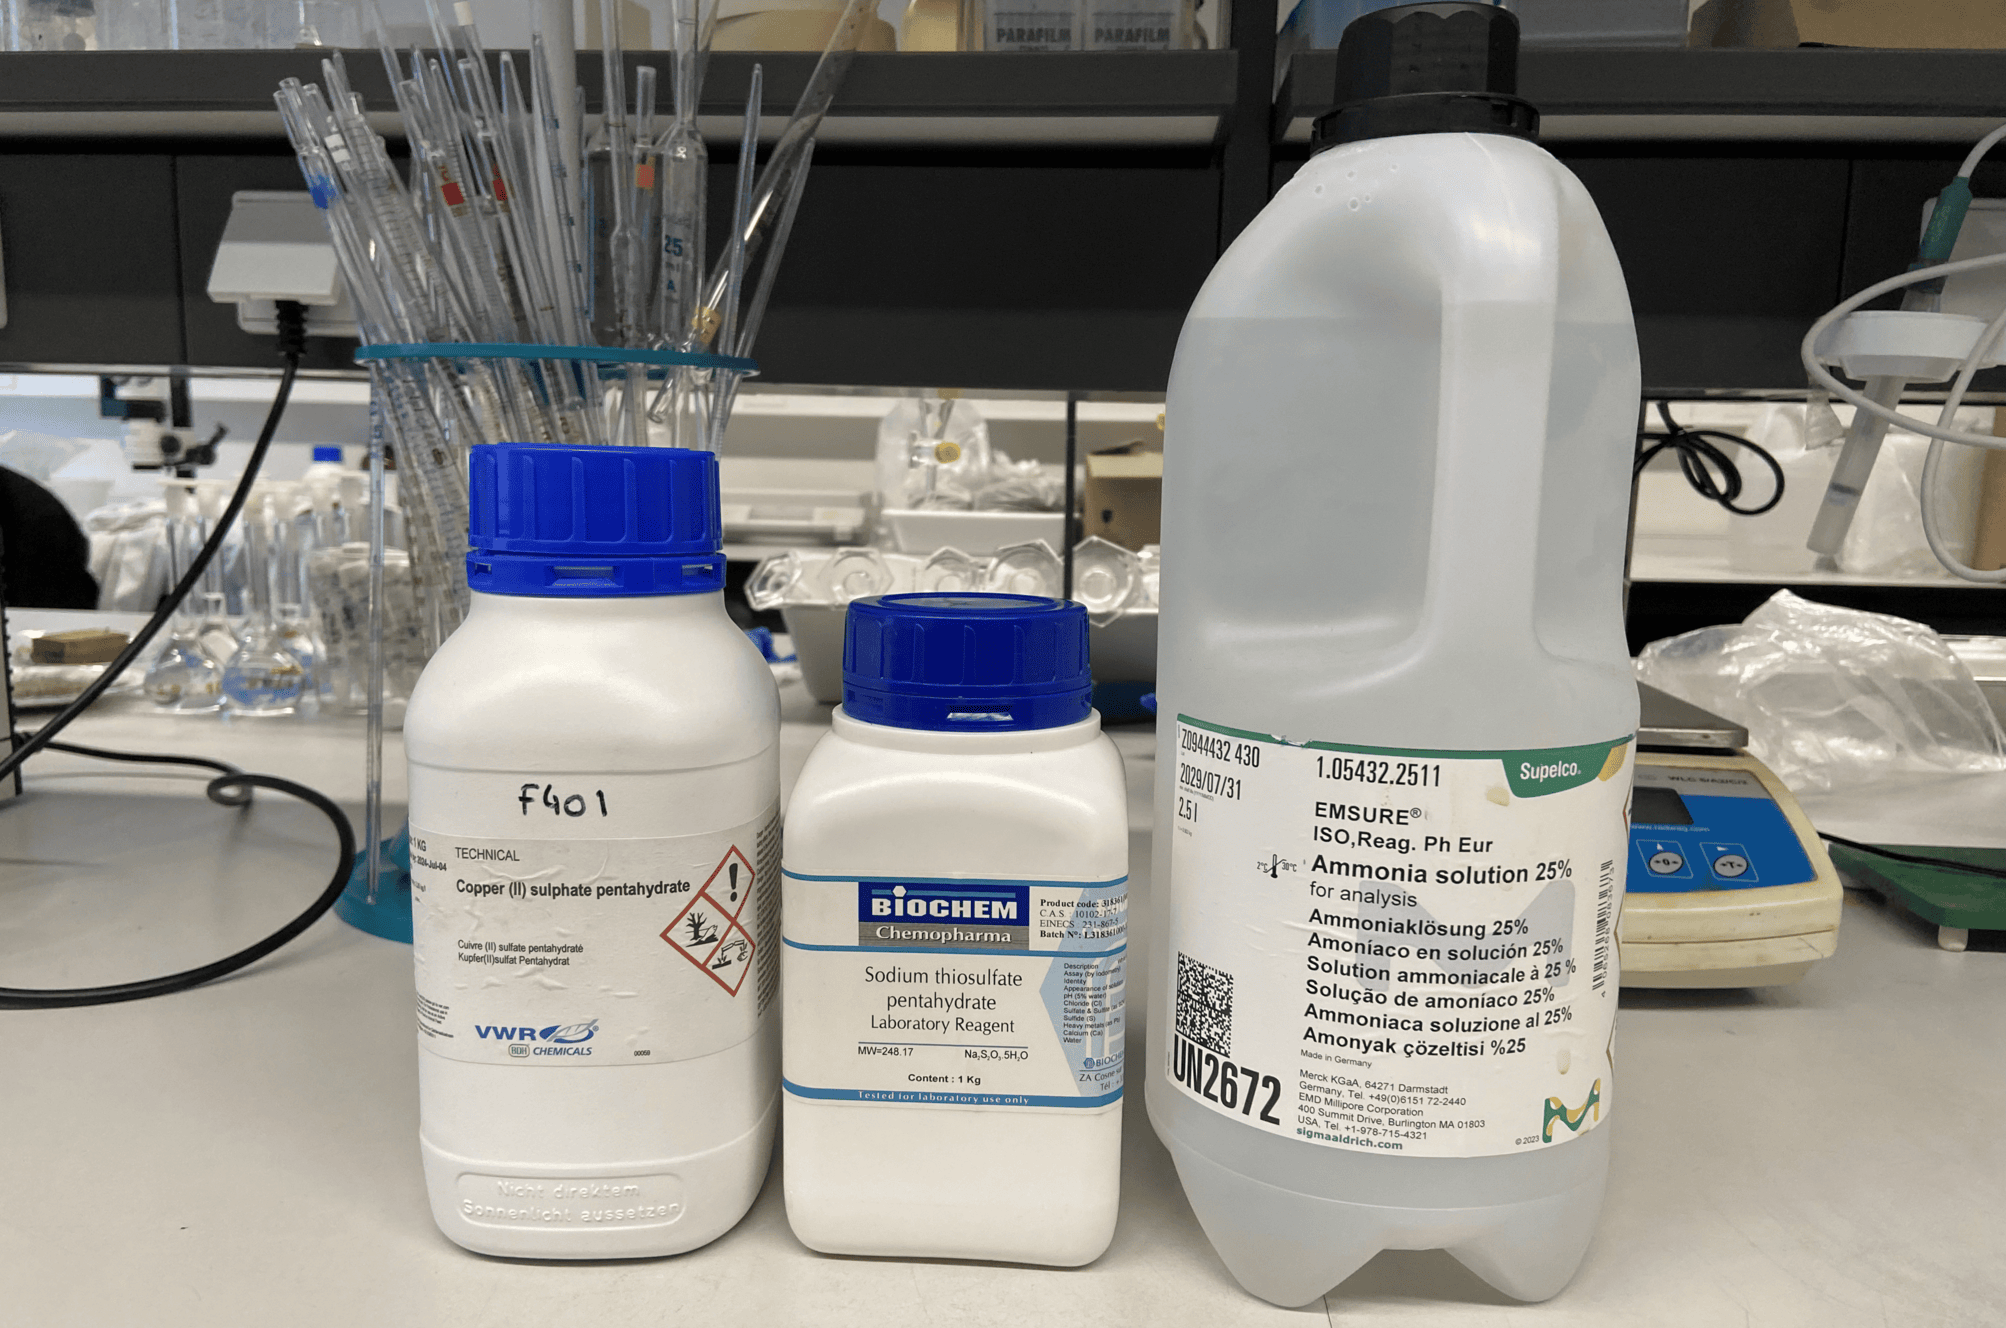
\includegraphics[width=\linewidth]{figures/reagentes-lixiviação 1}
    \caption{Reagentes utilizados na lixiviação.}
    \label{fig:reagentes-lixiviacao-1}
\end{marginfigure}

Num balão volumétrico de 250~mL foi colocado 15~mL de \AMO{}, com uma pipeta de 10~mL\@.
O volume restante foi preenchido com água destilada, até perfazer os 250~mL do balão.
Num gobelé, foi medida a massa de \TSP{} (99,34~g) e a massa de \SCP{} (1,01~g) que vão ser utilizados.
De seguida, juntou-se os conteúdos do balão volumétrico (água + \AMO{}) ao gobelé com o \TSP{} e \SCP{}, agitou-se com uma vareta de vidro até estar bem dissolvido e homogeneizado.

Foi medida a massa de minério a ser lixiviada (200,00~g), da amostra \texttt{A08.3}.
O minério foi colocado dentro do reator de borossilicato.
Adicionou-se ao reator a solução com os reagentes dissolvidos e acrescentou-se 150~mL de água de forma a perfazer os 400~mL de fase líquida, respeitando a relação S/L\@.

\begin{marginfigure}[-8\baselineskip]
    \centering
    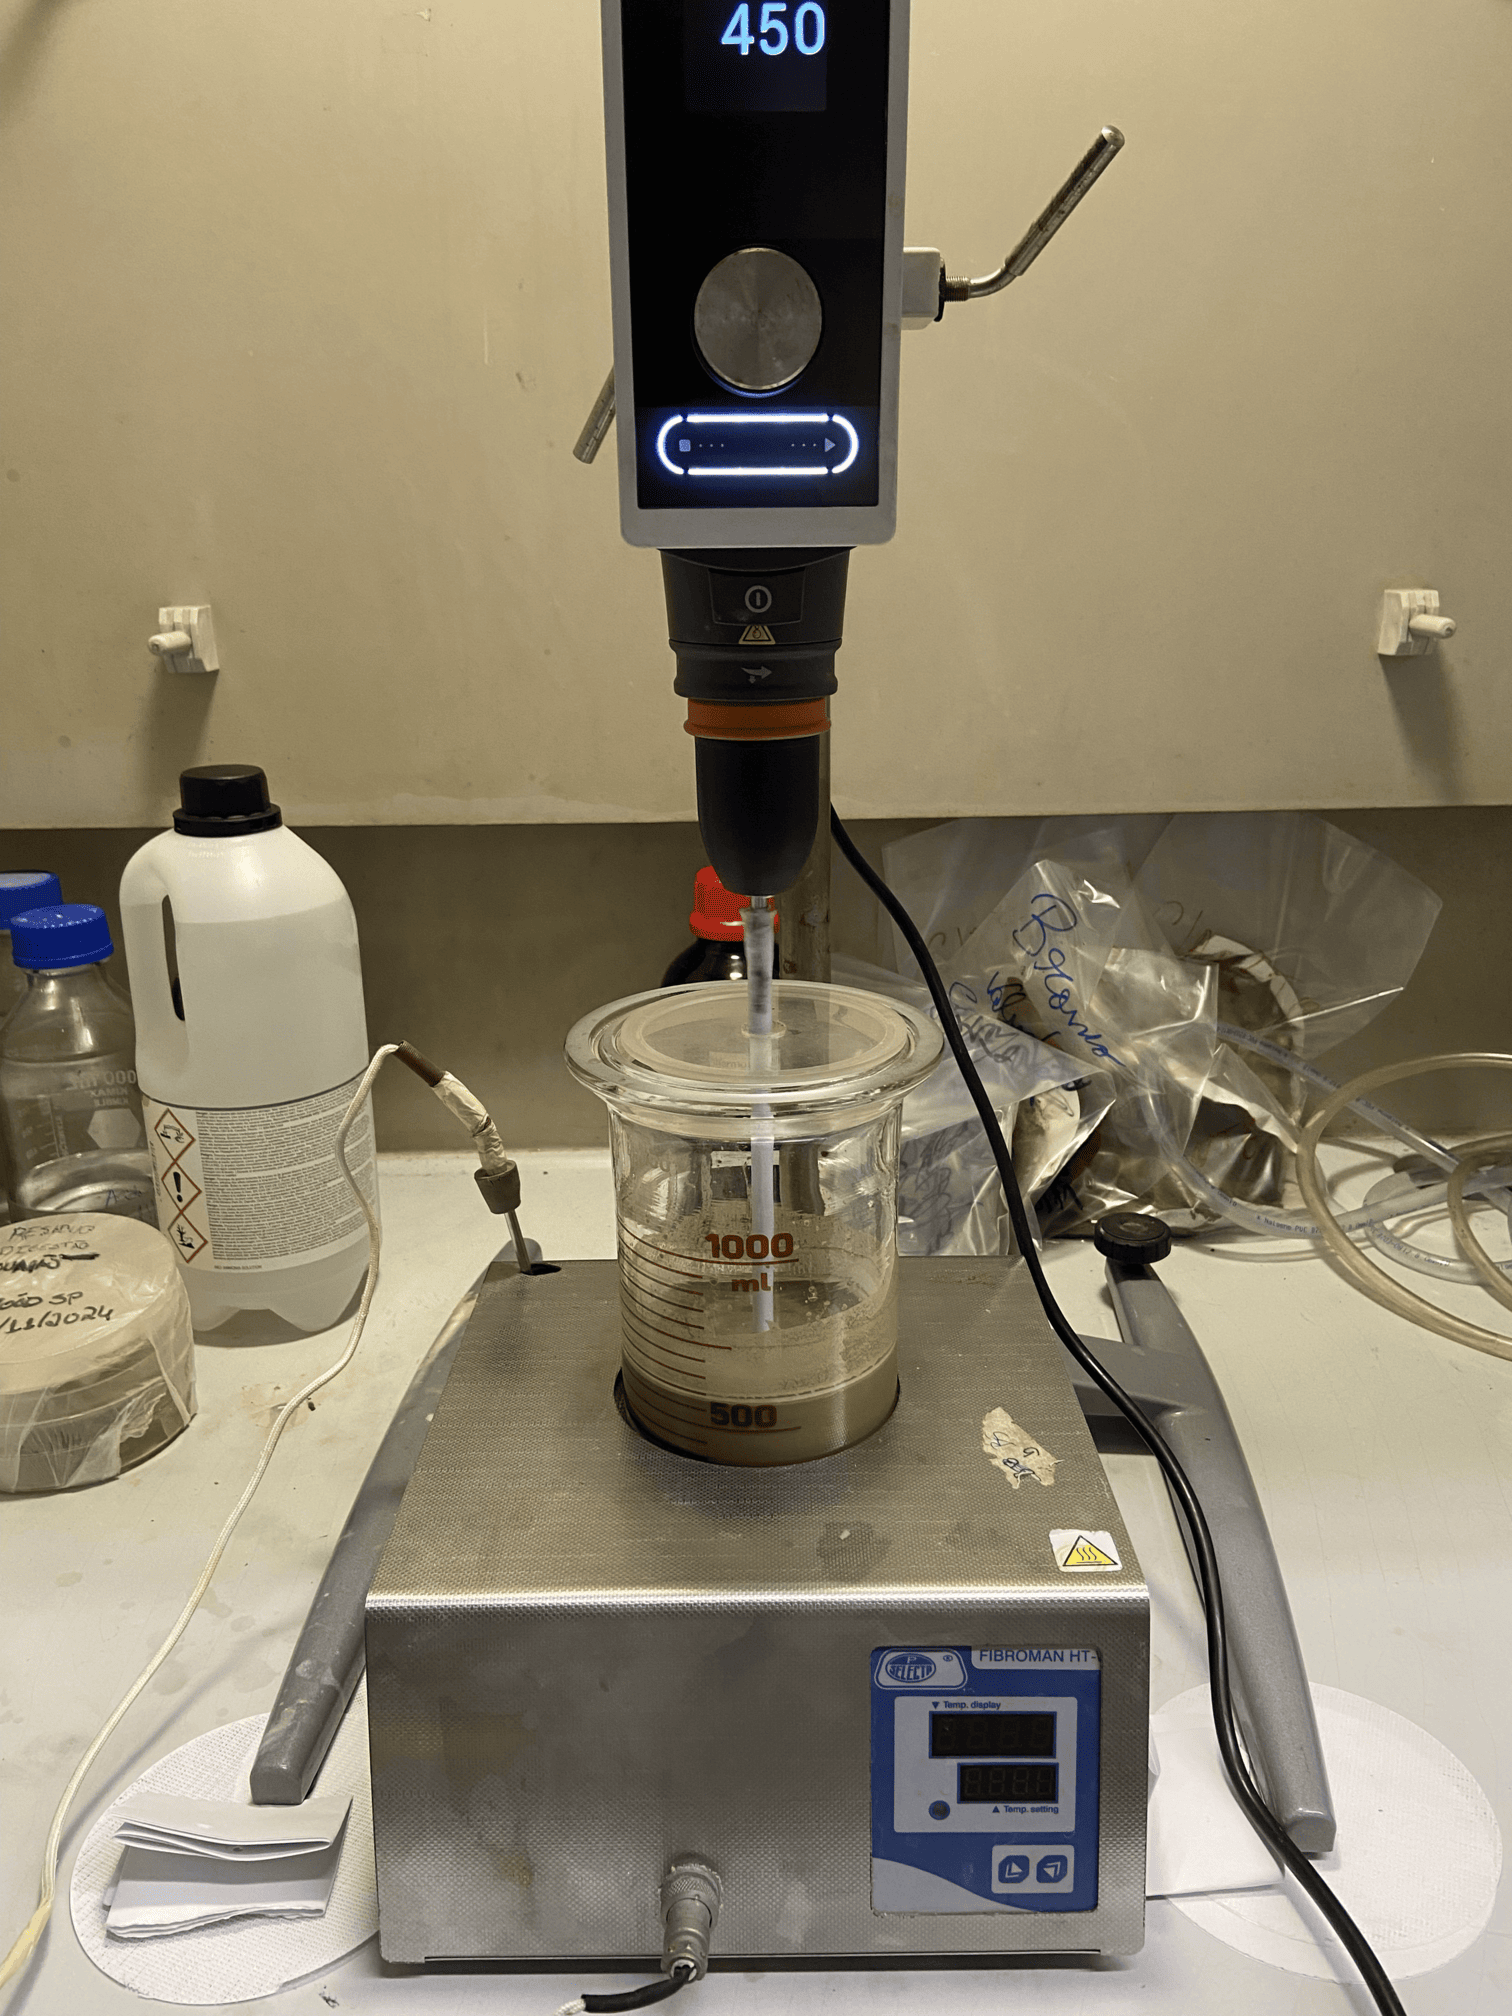
\includegraphics[width=0.9\linewidth]{figures/lixiviação-1 a decorrer}
    \caption{Lixiviação a decorrer.}
    \label{fig:lixiviacao1-a-decorrer}
\end{marginfigure}

Regulou-se o agitador e definiu-se uma velocidade de rotação de 450~rpm.
Deixou-se a trabalhar durante cerca de 5~minutos.
De seguida, parou-se o agitador, deixou-se decantar um pouco e mediu-se o pH (7,25) e o Eh (-86,0~mV - valor medido; 133~mV - valor convertido).

Uma vez registados os valores de pH e Eh, retomou-se o funcionamento do agitador.

\marginnote[-1\baselineskip]{Os valores de pH e de Eh não são fidedignos. Os equipamentos de medição não estavam calibrados, portanto os valores medidos podem não ser os valores reais.}

Deixou-se a lixiviar durante 8~horas.
No fim da lixiviação, mediu-se novamente o pH (6,15) e o Eh (-60,5~mV - valor medido; 159~mV - valor convertido).

De seguida, montou-se o sistema de filtragem, composto por um filtro de Büchner, um Kitasato, uma bomba de vácuo e um papel de filtro.
Filtrou-se e mediu-se o volume do licor de lixiviação - 369~mL\@.

\begin{marginfigure}
    \centering
    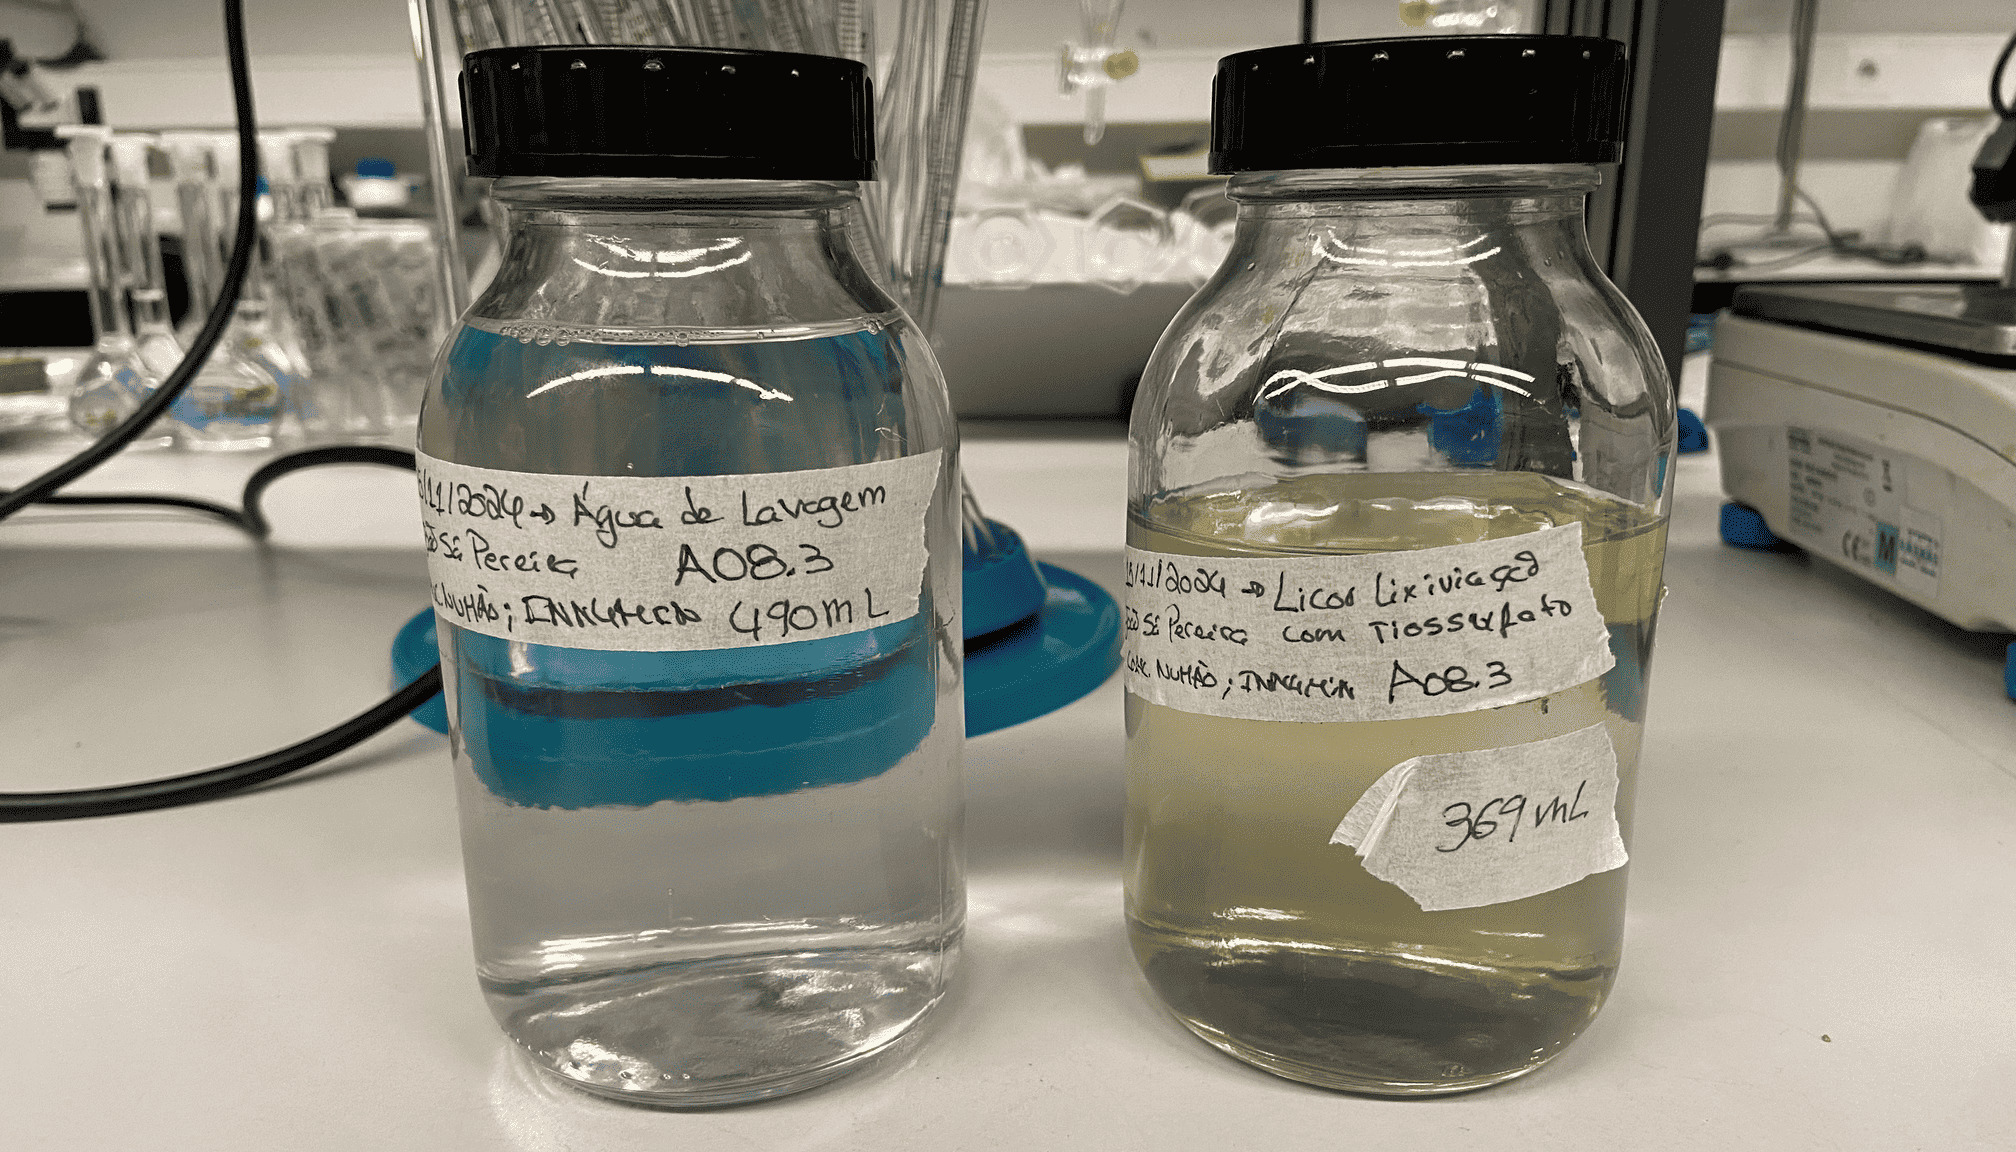
\includegraphics[width=0.9\linewidth]{figures/licor e agua lavagem lix tiossulfato}
    \caption{Licor de lixiviação e água de lavagem (Tiossulfato).}
    \label{fig:licor-lix-agua-lavagem-tiossulfato}
\end{marginfigure}

O resíduo sólido que foi filtrado foi lavado com 500~mL de água.
Colocou-se o resíduo de novo no reator, adicionou-se 500~mL de água e ligou-se o agitador, deixando lavar durante 30~minutos.

Após os 30~minutos, filtrou-se novamente o material.
Mediu-se o volume de solução de água de lavagem - 490~mL\@.

Tanto o licor de lixiviação como a água de lavagem, foram colocados em recipientes de vidro, identificados e armazenados - Figura~\ref{fig:licor-lix-agua-lavagem-tiossulfato}.

\begin{marginfigure}
    \centering
    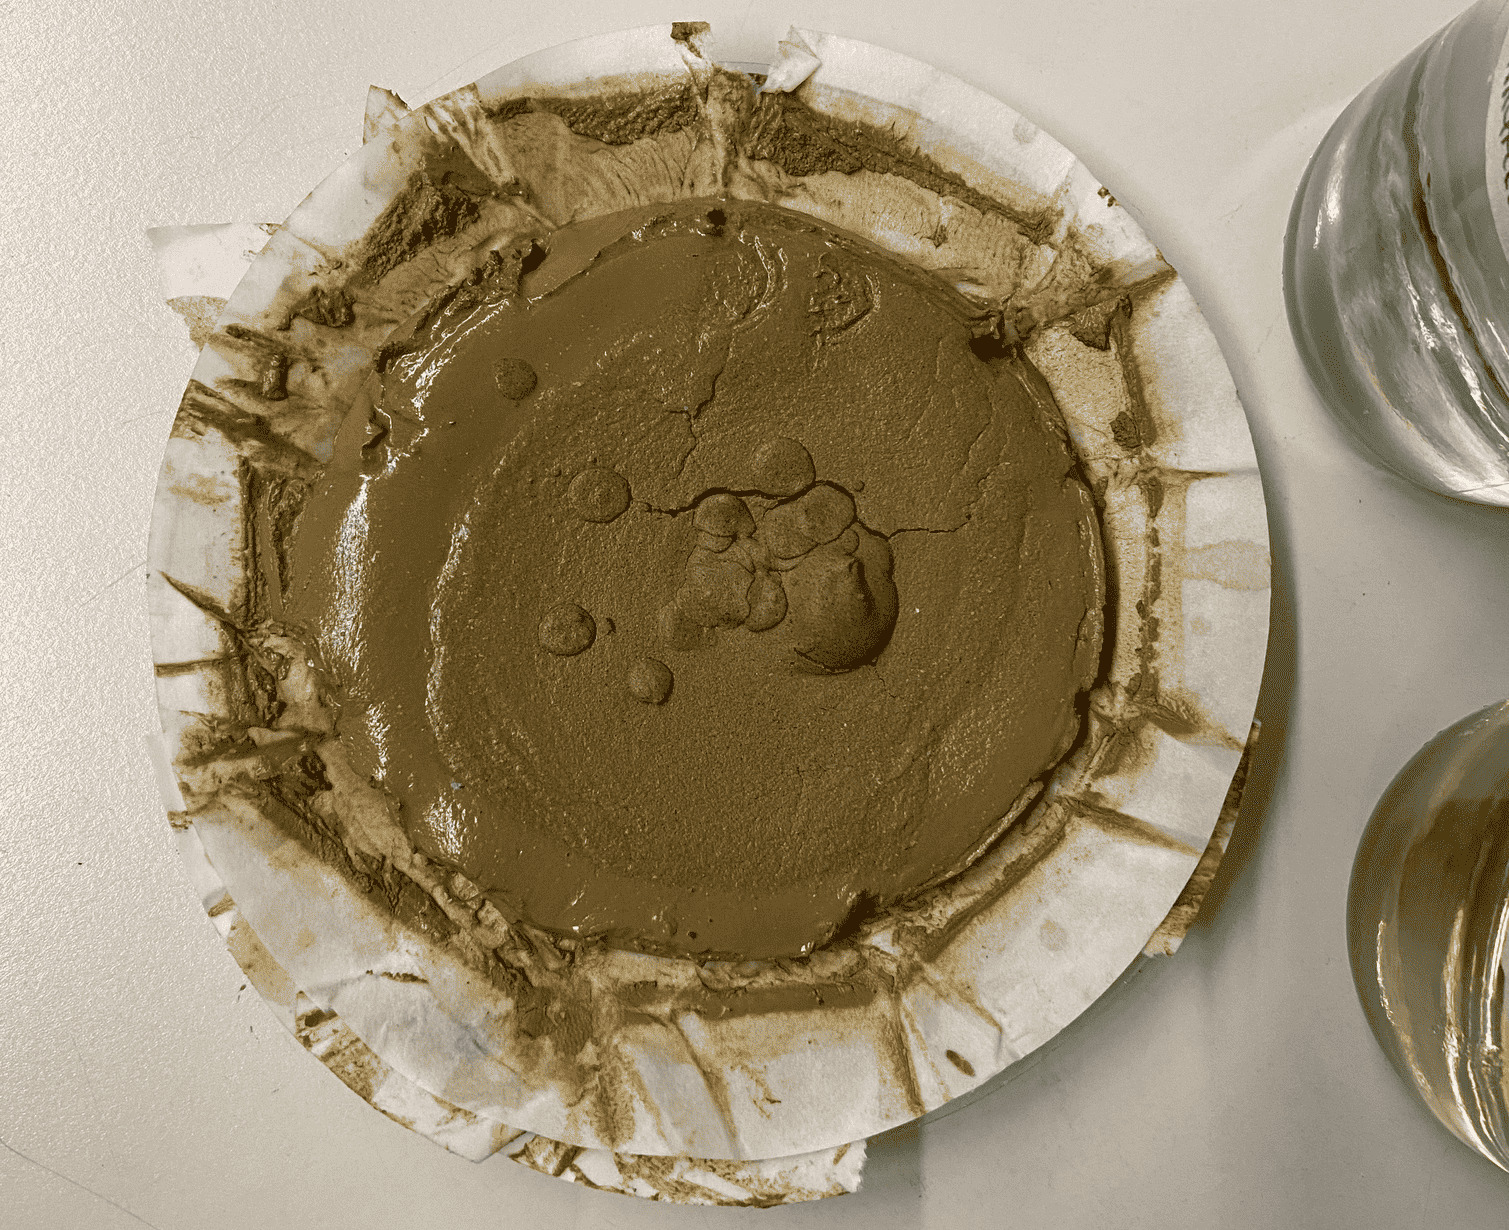
\includegraphics[width=0.9\linewidth]{figures/residuo_sol_lix_tiossulfato}
    \caption{Resíduo sólido da lixiviação (Tiossulfato).}
    \label{fig:res-solido-lix-tiossulfato}
\end{marginfigure}

O material, já lavado e filtrado (Figura~\ref{fig:res-solido-lix-tiossulfato}), foi colocado numa estufa a secar durante o fim-de-semana.
Após estar seco, mediu-se a massa - 192,61~g (já a descontar a massa do vidro de relógio e do papel de filtro).
Reservou-se.

\hrulefill

%%%%%%%%%%%%%%%%%%%%%%%%%%%%%%%%%%%%%%%%%%%%%%%%%%%%%%%%

\newday{19 Novembro 2024}\label{day:19-novembro-2024}

Hoje preparou-se o resíduo sólido da lixiviação para se realizar a digestão ácida.
O resíduo sólido proveniente da lixiviação com \TSP{}, foi moído no moinho de anéis.

Foram retirados 50~g de material, com o divisor de amostras\sidenote{Ver Figura~\ref{fig:divisor_de_amostras_retsch}.} tendo sido colocado 10~g em cinco copos distintos\sidenote{Ver procedimento do dia~\nameref{day:7-novembro-2024}.}.
Esses copos foram colocados na mufla e aquecidos até 700~\graus{} e deixados a arrefecer durante a noite.


\hrulefill

\newpage

\newday{20 Novembro 2024}

Hoje realizou-se a digestão ácida do resíduo de lixiviação com \TSP{}, dando seguimento ao dia~\nameref{day:19-novembro-2024}.

Foi seguido o mesmo procedimento do dia~\nameref{day:8-novembro-2024}.
\marginnote{Ver o procedimento em detalhe para mais informação.}

Utilizou-se a mesma relação de ácido sulfúrico e ácido nítrico, 1:3.
Ou seja, 6~mL de \ce{HNO3} e 18~mL de \ce{HCl}.
Foram feitos 3 ataques, com 1~hora e 30~minutos entre cada um.
Totalizando em 4~horas e 30~minutos de digestão.

No fim dos 3~ataques, juntou-se 4~mL de \ce{HCl} a cada um dos copos e verteu-se para balões volumétricos de 50~ml, separando o resíduo sólido do líquido.
O volume restante dos balões foi preenchido com água destilada.
O resíduo sólido foi colocado numa placa de Petri e reservado.

Posteriormente, o conteúdo dos balões volumétricos será filtrado para ser analisado na absorção atómica.

\hrulefill

%%%%%%%%%%%%%%%%%%%%%%%%%%%%%%%%%%%%%%%%%%%%%%%%%%%%%%%%

\newday{22 Novembro 2024}

Hoje realizou-se a lixiviação com Tioureia (\tio{}) de um dos restantes sacos de $\approx$~250~g da amostra \texttt{A08}.
O saco selecionado, aleatoriamente, foi a sub-amostra \texttt{A08.4}.

Para a elaboração do procedimento desta lixiviação, foi tomado em consideração o artigo ``\emph{An innovative thiourea gold leaching process}''\cite{innovative_thiourea_1998}.
A partir deste artigo foram definidas as concentrações dos reagentes a usar e o procedimento a ser tomado para a lixiviação.

Nesse sentido, as concentrações utilizadas foram as seguintes:
\begin{itemize}
    \item[-] Tioreia, \tio{} - 100~g/kg de minério;
    \item[-] Sulfato de ferro (III) pentahidratado, \sulfe{} - 0,5~g/kg de minério;
    \item[-] Ácido sulfúrico, \acsul{} - o necessário para obter uma solução com pH = 1.
\end{itemize}

Foi decidido utilizar 100~g de minério da sub-amostra \texttt{A08.4}, para a lixiviação. 
A lixiviação será feita com uma razão sólido líquido de 1 para 5 (S/L = 1/5).

A lixiviação foi efetuada a temperatura ambiente, com uma agitação de 350~rpm, durante 6~horas.
Foi utilizado um reator de borossilicato de 500~mL.

Foi realizado o cálculo da quantidade de reagentes necessários, para as concentrações estipuladas. 
Para o caso do sulfato de ferro (III), como a concentração utilizada no artigo era muito baixa, utilizou-se sulfato de ferro (III) pentahidratado. Portanto, ajustou-se os cálculos tendo em consideração esta alteração.

A quantidade de reagentes utilizada foi a seguinte:
\begin{itemize}
    \item[-] \tio{} - 10~g;
    \item[-] \sulfe{} - 0,0612~g;
    \item[-] \acsul{} - 1,85~mL\marginnote{O ácido sulfúrico foi adicionado, pouco a pouco, no reator em agitação com apenas tioureia dissolvida. Foi-se medindo o pH à medida que se ia adicionando \acsul{} até que a solução se apresentou com pH de 1,3.}.
\end{itemize}

No reator de borossilicato, foi adicionado 500~mL de água destilada e 10~g de \tio{].
Dissolveu-se a tioureia com auxílio do agitador mecânico e ajustou-se o pH, adicionando 1,85~ml de \acsul{}, o que resultou num pH = 1,3.
Após acidificar a solução, adicionou-se \sulfe{} e o minério no reator, regulando o agitador para 350~rpm e dando início à lixiviação às 10h18.

Foi-se verificando o pH ao longo da lixiviação para garantir que a solução se encontrava com um pH = 1, adicionando \acsul{} conforme necessário.

\begin{marginfigure}
    \centering
    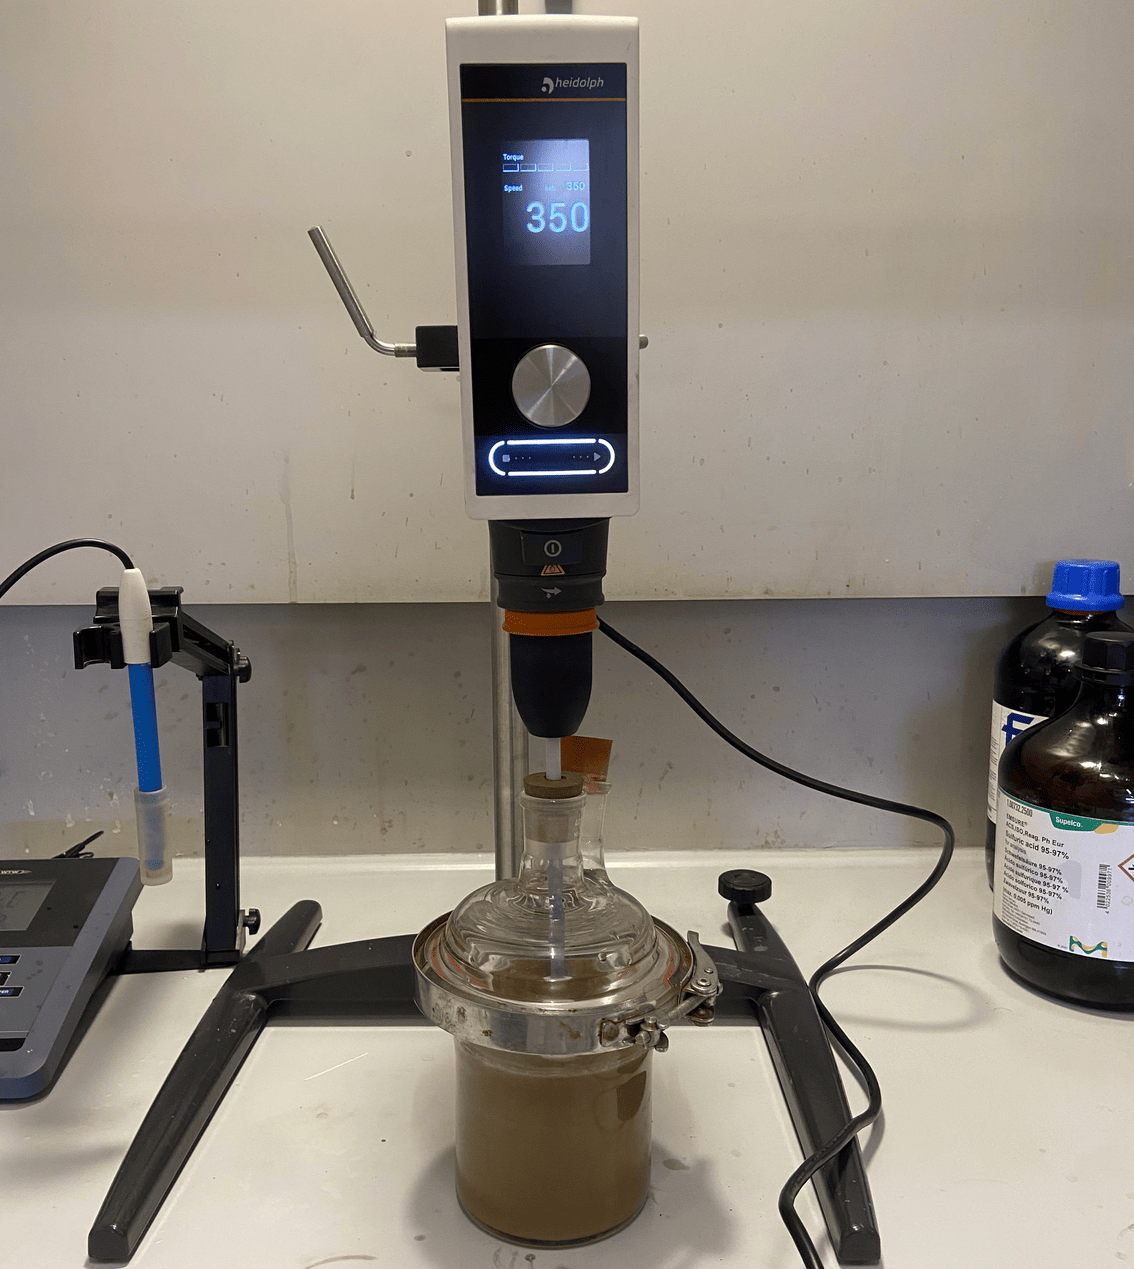
\includegraphics[width=0.9\linewidth]{figures/Lixiviação - Tioureia.png}
    \caption{Lixiviação com tioureia a decorrer.}
    \label{fig:lix-tioureia-a-decorrer}
\end{marginfigure}

Adicionou-se, durante as 6~horas de lixiviação, 1,465~mL de \acsul{}.
No total adicionou-se 3,315~mL de \acsul{}, sendo que 1,85~mL foi adicionado antes da lixiviação, sem o minério na solução e 1,465~mL foi adicionado durante a lixivição, com o minério na solução.

Foi preparada uma solução de lavagem com água destilada acidificada (pH = 1).
A relação S/L para a lavagem foi de 1/2,5. 
Portanto, para 100~g de minério utilizou-se 250~mL de água destilada acidificada.
Para acidificar 250~mL de água destilada, adicionou-se 1~mL de \acsul{} resultando num pH = 1,046.

Uma vez terminada a lixiviação, filtrou-se o material com um sistema de filtração composto por um filtro Büchner, um balão Kitasato, um papel de filtro e uma bomba de vácuo. 
Filtrou-se a solução, mediu-se o volume de licor filtrado (473~mL) e mediu-se o pH do licor (1,195).

\begin{marginfigure}
    \centering
    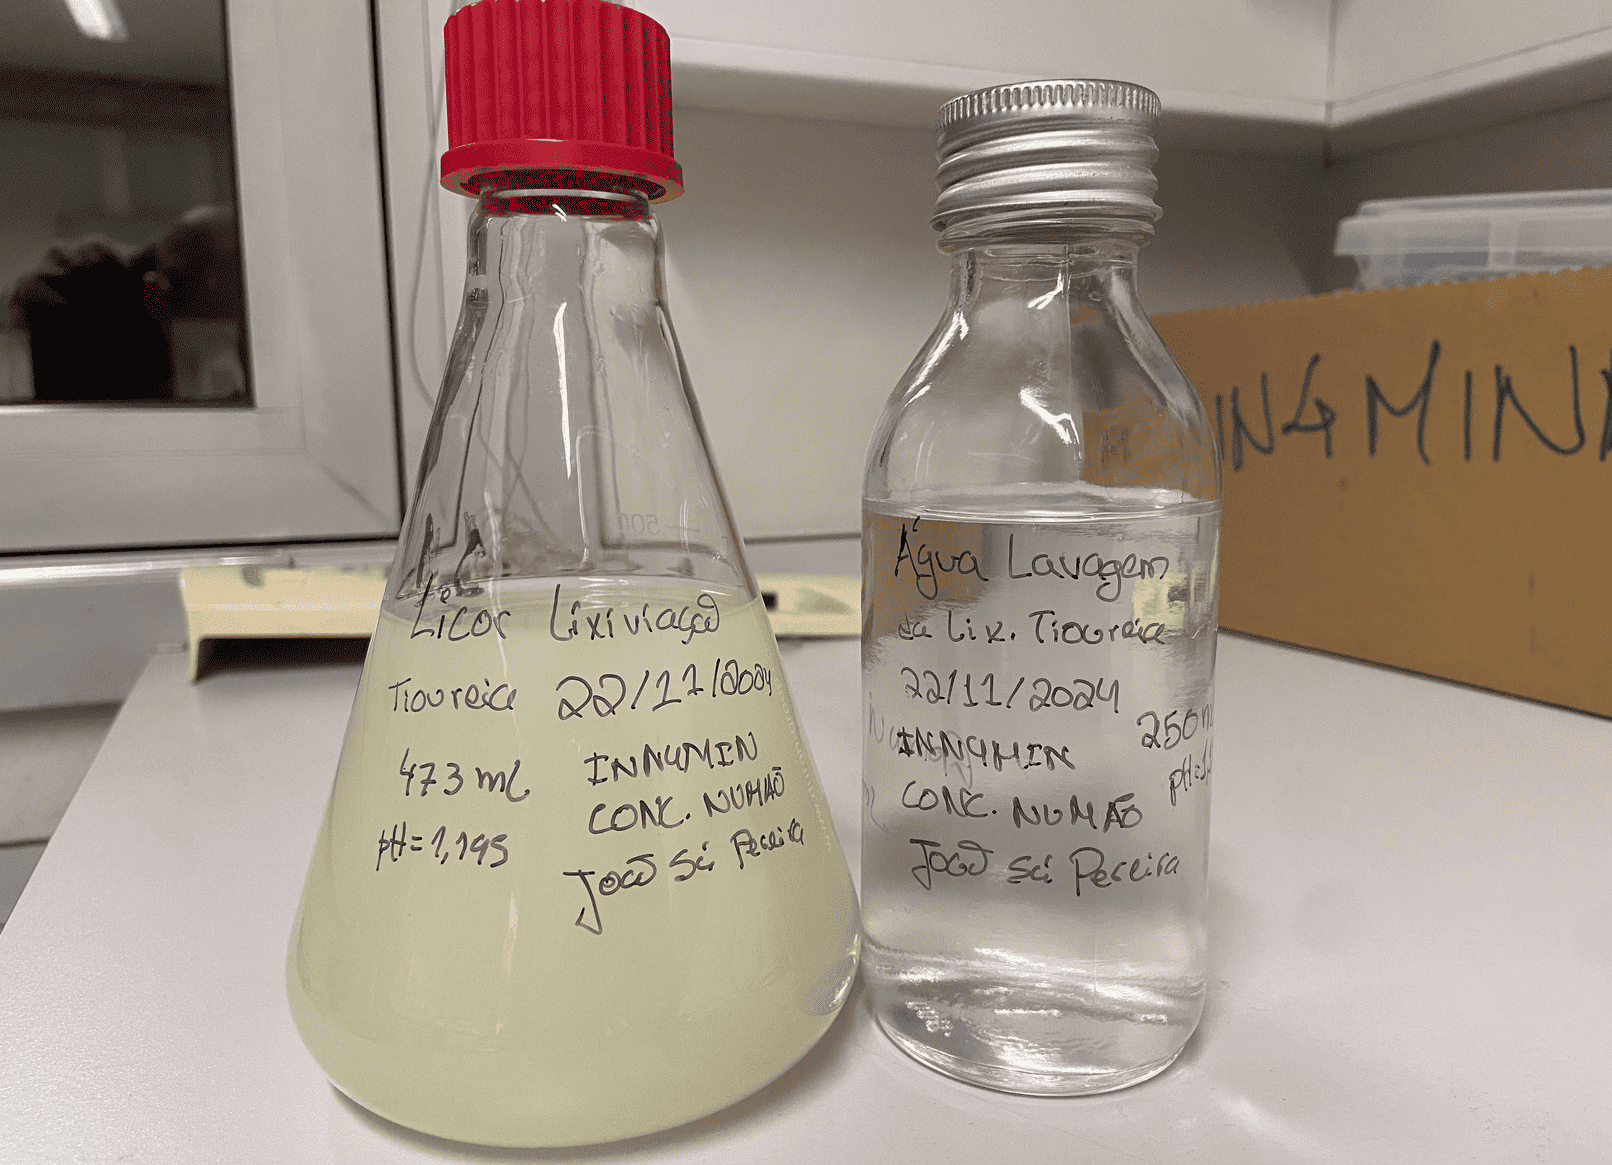
\includegraphics[width=0.9\linewidth]{figures/Lixiviação Tioureia (Licor e Água de Lavagem).png}
    \caption{Licor de lixiviação e água de lavagem (Tioureia).}
    \label{fig:licor-agualavagem-tioureia}
\end{marginfigure}

Colocou-se o sólido filtrado novamente no reator de borossilicato, adicionou-se os 250~mL de água destilada acidificada e deixou-se a lavar durante 30~minutos com o agitador mecânico a 350~rmp.
Uma vez terminada a lavagem, filtrou-se novamente com o mesmo sistema de filtragem.
Mediu-se o volume da água de lavagem (250~mL) e mediu-se o pH (1,118).

Tanto o licor de lixiviação como a água de lavagem, foram colocados em recipientes de vidro, identificados e armazenados - Figura~\ref{fig:licor-agualavagem-tioureia}.

O sólido filtrado foi colocado numa placa de Petri e deixado a secar na estufa a 60~\graus{} durante 8~horas.
O resíduo sólido ficou dentro da estufa (desligada), durante o fim de semana.
O papel de filtro utilizado nas duas filtragens, pesavam 2,40~g e 2,33~g. \marginnote{Não esquecer de remover estes valores quando se for medir a massa do resíduo sólido seco.}

Após estar seco, mediu-se a massa - \emph{inserir massa} (já a descontar a massa do vidro de relógio e do papel de filtro) . 
Reservou-se.

\hrulefill

%%%%%%%%%%%%%%%%%%%%%%%%%%%%%%%%%%%%%%%%%%%%%%%%%%%%%%%%